%%%%%%%%%%%%%%%%%%%%%%%%%%%%%%%%%%%%%%%%%%%%%%%%%%%%%%%%%%%%%%%%%%%%%%%%%%%%%%%%
%2345678901234567890123456789012345678901234567890123456789012345678901234567890
%        1         2         3         4         5         6         7         8

%\documentclass[letterpaper, 10 pt, conference]{ieeeconf}  % Comment this line out
                                                          % if you need a4paper
%\documentstyle[10pt,times,psfig,twocolumn]{article}
\documentclass[letterpaper, 10pt, conference]{ieeeconf}      % Use this line for a4
\usepackage{xcolor}                                                 % paper

\IEEEoverridecommandlockouts                              % This command is only
                                                          % needed if you want to
                                                          % use the \thanks command
\overrideIEEEmargins
% See the \addtolength command later in the file to balance the column lengths
% on the last page of the document

\usepackage{graphicx}

% The following packages can be found on http:\\www.ctan.org
%\usepackage{graphics} % for pdf, bitmapped graphics files
%\usepackage{epsfig} % for postscript graphics files
%\usepackage{mathptmx} % assumes new font selection scheme installed
%\usepackage{times} % assumes new font selection scheme installed
%\usepackage{amsmath} % assumes amsmath package installed
%\usepackage{amssymb}  % assumes amsmath package installed

\title{\LARGE \bf
Automating Interictal Spike Detection: Revisiting A Simple Threshold Rule
}

\author{Palepu A.$^{1}$, Premanathan S.$^{1}$, Azhar, F.$^{3}$, Vendrame, M.$^{4}$, Loddenkemper, T.$^{5}$, Reinsberger, C.$^{4}$,  Kreiman, G.$^{6}$  \\ 
Parkerson, K.A.$^{4}$, Sarma, S. {\it IEEE Member}$^{1}$, and Anderson, W.S.$^{2}$%
\thanks{$^{1}$Institute for Computation Medicine, Johns Hopkins University, Baltimore, MD, U.S.A.}
\thanks{$^{2}$Department of Neurosurgery, The Johns Hopkins Hospital, Baltimore, MD, U.S.A.}
\thanks{$^{3}$Department of Neurosurgery, Brigham and Women\'s Hospital, Harvard Medical
School, Boston, MA, U.S.A.}
\thanks{$^{4}$Department of Neurology, Brigham and Women\'s Hospital, Harvard Medical School,
Boston, MA, U.S.A.}
\thanks{$^{5}$Department of Neurology, Children\'s Hospital Boston, Harvard Medical School,
Boston, MA, U.S.A.}
\thanks{$^{6}$Department of Ophthalmology, Children\'s Hospital Boston, Harvard Medical School,
Boston, MA, U.S.A.}
}


\begin{document}



\maketitle
\thispagestyle{empty}
\pagestyle{empty}


%%%%%%%%%%%%%%%%%%%%%%%%%%%%%%%%%%%%%%%%%%%%%%%%%%%%%%%%%%%%%%%%%%%%%%%%%%%%%%%%
\begin{abstract}

Interictal spikes (IIS) are bursts of neuronal depolarization observed electrographically between periods of seizure activity in epilepsy patients. However, IISs are difficult to characterize morphologically and their effects on neurophysiology and cognitive function are poorly understood. Currently, IIS detection requires laborious manual assessment and marking of electroencephalography (EEG/iEEG) data. This practice is also subjective as the clinician has to select the mental threshold that EEG activity must exceed in order to be considered a spike. The work presented here details the development and implementation of a simple automated IIS detection algorithm. This preliminary study utilized intracranial EEG recordings collected from 7 epilepsy patients, and IISs were marked by a single physician for a total of 1339 IISs across 68 active electrodes. The proposed algorithm implements a simple threshold rule that scans through iEEG data and identifies IISs using various normalization techniques that eliminate the need for a more complex detector. The efficacy of the algorithm was determined by evaluating the sensitivity and specificity of the detector across a range of thresholds, and an approximate optimal threshold was determined using these results. With an average true positive rate of over 98\% and a false positive rate of below 2\%, the accuracy of this algorithm speaks to its use as a reliable diagnostic tool to detect IISs, which has direct applications in localizing where seizures start, detecting when seizures start, and in understanding cognitive impairment due to IISs. Furthermore, due to its speed and simplicity, this algorithm can be used for real-time detection of IIS that will ultimately allow physicians to study their clinical implications with high temporal resolution and individual adaptation.

\end{abstract}


%%%%%%%%%%%%%%%%%%%%%%%%%%%%%%%%%%%%%%%%%%%%%%%%%%%%%%%%%%%%%%%%%%%%%%%%%%%%%%%%
\section{INTRODUCTION}

The paroxysmal nature of interictal spikes (IISs) and their manifestation as large amplitude, high frequency neurophysiological waveforms~\cite{c2} makes them particularly strong candidates as potential markers of epileptogenesis. Interictal spikes (example shown in Fig. ~\ref{fig1}), are commonly observed through either scalp electroencephalography (EEG) or intracranial electroencephalography (iEEG) recordings of epileptic patients. The diagnostic utility conferred by EEG originates from its high temporal resolution, allowing physicians to identify, in real time, patterns or irregularities in the dynamic electrical activity that occurs within the brain. 

\begin{figure}[t!]
    \centering
    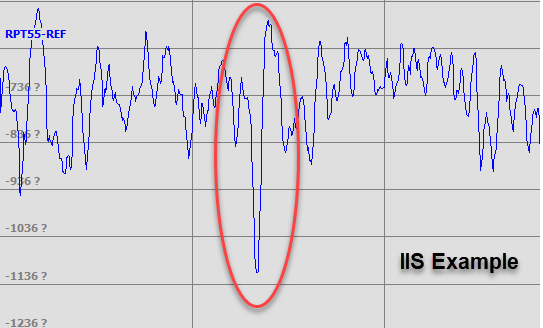
\includegraphics[height=1.5in, width=3.5in]{IISExample.png}
    \caption{An example of an interictal spike. These spikes are brief ($<$250 millisecond) morphological events in an EEG recording that occur in between periods of epileptic seizure.}
    \label{fig1}
\end{figure}

The effects of IISs on various facets of neuronal processing continue to elude physicians and the scope of these effects remains unknown. Critical to elucidating the pathological effects of IISs is developing a uniform method of characterizing and detecting them~\cite{c5}. IISs are currently manually annotated by clinicians who visually inspect scalp EEG data or iEEG data. Scalp EEG recordings inherently exhibit poor spatial resolution and a reduced signal-to-noise ratio~\cite{c12}. Intracranial EEG (iEEG), though an invasive procedure, produces waveforms with a higher spatial resolution and signal-to-noise ratio than that of scalp EEG, permitting better localization and detection of IISs. Despite the advantages of iEEG, annotation of IISs is an arduous process subject to error and varied results since each physician must visually determine, based on individual experience and knowledge, which abnormal waveforms appear to be IISs and which do not. 

As a result, several automated IIS detection algorithms have been proposed to combat variability in IIS annotations and have the potential to provide a more consistent and efficient detection framework. Previously, it was thought that a threshold detector was insufficient to accurately detect IISs, with some initial detectors yielding a sensitivity of only 63.4\%~\cite{c6}. As a result, more computationally complex algorithms have been developed to compensate for the poor performance of simple threshold detectors. Some of these algorithms employ template-matching techniques, which are capable of locating IISs quickly and accurately. El-Gohary et al. \cite{c4} reported a template-matching algorithm that achieved a sensitivity of 96\%. However, these algorithms require a physician to mark a few examples of IISs in the data before application of the algorithm itself.

Other techniques utilize dimensionality reduction methods via neural networks to transform several context parameters, such as components of EEG waveforms, into a much smaller collection of parameters that more precisely capture various patterns in EEG activity~\cite{c8}. One such algorithm used by Tarassenko et al. \cite{c10} achieved a sensitivity and specificity of 87\% and 96\%, respectively, but took over twenty minutes to analyze what a threshold detector could analyze in approximately ten seconds. Furthermore, the determination of which parameters to consider in the classification of interictal spikes by a neural network remains subjective. Other procedures approach interictal spike detection using mathematically intricate decompositions of waveforms that ultimately fail to establish a uniform definition of the morphological and physiological nature of interictal spikes. 

While the aforementioned algorithms have considerably advanced the use of computational techniques to address the need for automated spike detection~\cite{c1,c11,c3}, the algorithm proposed here revisits the simple threshold rule as it remains the computationally least taxing. Specifically, we discuss the development and implementation of an automated IIS detection algorithm that is able to rapidly analyze iEEG data and locate interictal spikes without the need for preliminary annotations made by the physician. This algorithm utilizes a novel normalization scheme to preprocess the data and then a threshold detector is applied to obtain an optimal threshold of neuronal activity that maximizes sensitivity and specificity of IIS detection. The algorithm was trained on raw iEEG data obtained from seven patients with epilepsy. Each patient contributed one hour of data, totaling to seven hours of raw intracranial EEG data obtained. A single physician reviewed the iEEG data and marked the time points at which any visually observed IISs occurred on each electrode contact in each patient.

\section{METHODS}

\subsection{Subjects and iEEG Recordings}
Patients included in this study were surgically treated for medically intractable seizures at the Brigham \& Women's epilepsy center. See Table~\ref{subjects} for patient details. All patients included in this study underwent invasive pre-surgical monitoring with subdural grid-and-strip arrays and possibly depth electrodes for seizure localization or mapping of eloquent areas. The research protocol was reviewed by the Brigham \& Women's Institutional Review Board (IRB). Digitized data was stored in an IRB-approved database compliant with Health Insurance Portability and Accountability Act (HIPAA) regulations.
 
As part of routine clinical care, up to three board-certified epileptologists marked, by consensus, the unequivocal electrographic onset of each seizure and the period between seizure onset and termination. The seizure onset was indicated by a variety of stereotypical electrographic features, which include, but were not limited to, the onset of fast rhythmic activity, an isolated spike or spike-and-wave complex followed by rhythmic activity, or an electrodecremental response. Concurrently with the examination of the EEG recordings, changes in the patients behavior were sought from the video segment of video-EEG recordings. For each patient, we combined surgical notes about the electrodes corresponding to resected regions and postoperative follow-up information about how the resection affected the patient's seizures.

iEEG recordings were acquired through subdural grid arrays or depth electrodes in various combinations as determined by clinical assessment for patients with temporal, parietal, or frontal lobe seizures, with 40-80 recording electrodes per patient. The recordings were taken over a total of seven days, and a single clinician chose an hour from each patient to annotate. This clinician viewed the seven hours of iEEG recordings and marked IISs as they presumably occurred. Across all seven patients, only 68 electrodes in total recorded interictal spike activity. Intracranial contact locations were documented by post-operative CT co-registered with a pre-operative MRI. %Signals were acquired using continuous multi-channel iEEG recordings collected over 5 days on average (min.: 2 days; max: 10 days). Clinical monitoring lasted 5-10 days per patient and included 2-7 clinical seizures. Then clinicians clipped what they deemed clean sets of data and passed it through a secure transfer for the data analysis.

\subsection{IIS Detection Algorithm}

The raw iEEG data was normalized and processed through the following procedure so that comparisons and manipulations of the data could be made across patients along a notionally common scale. Initially, a 60 Hz notch filter was applied in order to significantly reduce noise from the iEEG signals. Afterwards, the notch-filtered iEEG recordings, regardless of their measured raw values, were normalized to range $[-1, 1]$, where -1 represents the $x^{th}$ percentile and 1 represents the ($100-x^{th}$) percentile. $x$ is determined independently for each channel and is directly correlated with the standard deviation of the channel. Finally, a moving average for each channel across one second, or 250 data points, was subtracted from the data in order to eliminate the effect of a changing baseline.  In doing so, rapid shifts in the signal are accentuated while more gradual changes are diminished. These normalization steps are shown in Fig.~\ref{fig2} and Fig.~\ref{fig3}.

\begin{figure}[t!]
    \centering
    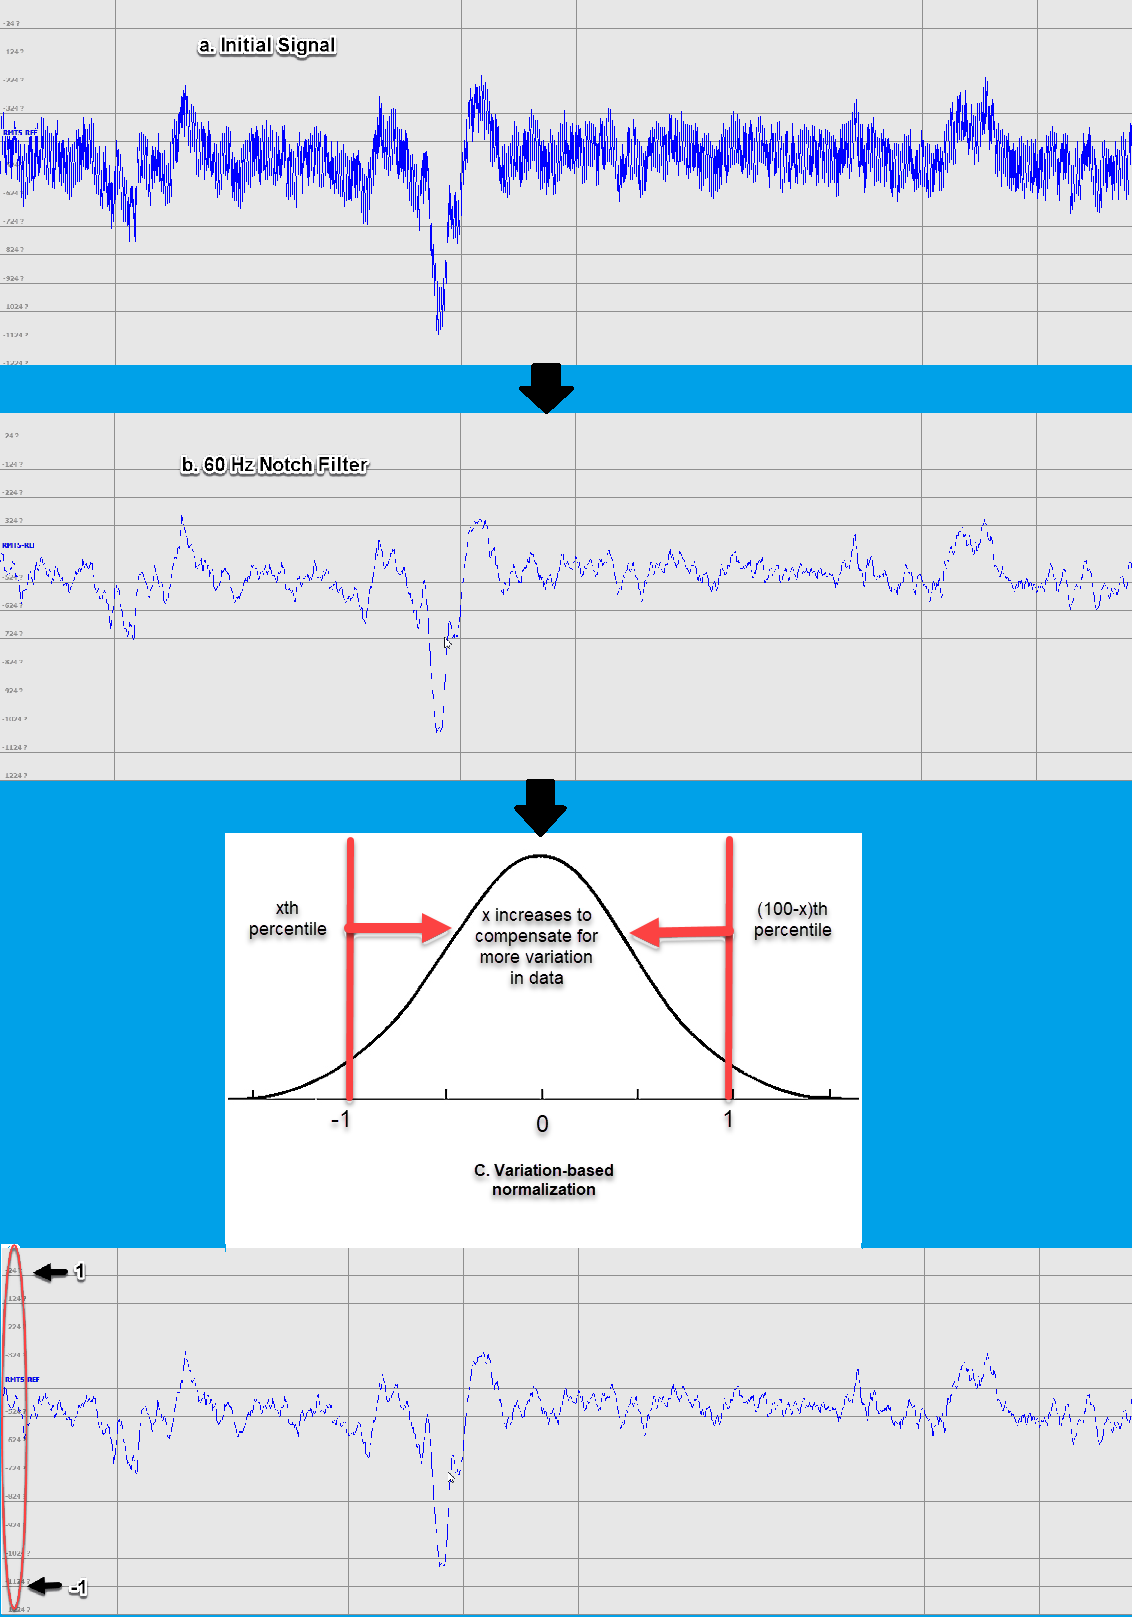
\includegraphics[height=3.5in, width=3.2in]{NormalizationTechniques.png}
    \caption{Normalization techniques used to remove noise and standardize data. (a) An example of raw iEEG signal from one of the patients. (b) The same signal as above after being passed through a notch filter with Q-factor of 20. (c) The variation-dependent normalization changes the scale of the signal to -1 to 1.}
    \label{fig2}
\end{figure}

\begin{figure}[t!]
    \centering
    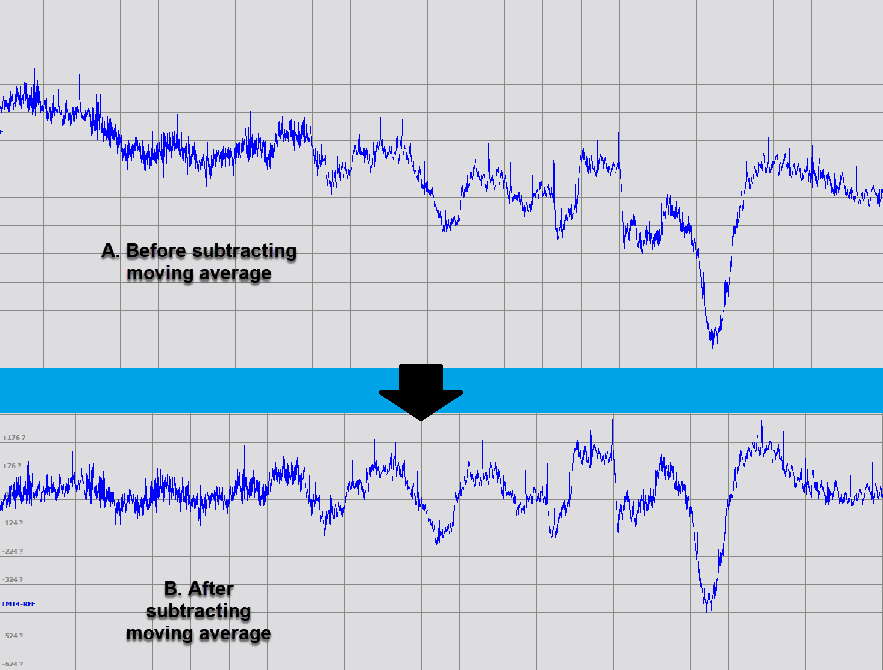
\includegraphics[height=2.2in, width=3.2in]{MovingAvgTechniques.png}
    \caption{Subtraction of the moving average. (a) An example of a channel with a dynamic baseline. (b) By subtracting a moving average from the data, spikes are preserved while the baseline becomes flat and more standardized.}
    \label{fig3}
\end{figure}

Once the iEEG data was processed using the aforementioned methods, the automated IIS detection algorithm, described in Fig.~\ref{fig4} was applied to the processed data. For each patient, 50\% of the time points at which voltage readings were taken, selected at random, served as the training data set that the algorithm would use to learn and infer a function from. If any channel had greater than twenty-five percent of its time points above an initial threshold of -0.5, then those channels were disregarded, ensuring that the algorithm was only detecting channels that had IISs as opposed to channels that were noisy. 

The algorithm was then used to determine the occurrence of IISs according to a specified threshold value. A very wide range of threshold values, from -0.3 to -0.7, in increments of 0.02, were chosen in order to ensure the optimal threshold would be captured somewhere in this range. If the time point at which the normalized iEEG voltage reading was between -1 and the specified threshold value, then that time point was marked as an IISs. 

In MATLAB, the occurrence of IISs was documented in the following manner: a two-dimensional array of zeroes was created in which the rows represented individual channels and the columns represented their time points. If an IIS was observed in a particular channel at a particular time point, a 1 was placed in the corresponding location of the two dimensional array. As follows, for each patient, a two-dimensional array was created detailing all of the channels in which IISs were observed as well as the time points that said IISs were observed at. We will call this two-dimensional array $X$. Physician-annotated spikes were processed in a similar fashion and recorded in another two-dimensional array that will be referred to as Y. A third two-dimensional array, $Z$, was created and set equal to $(2X)+Y$, such that for any statistical classification of a spike i, $i \in Z:i \in [0, 3],$ where a true positive result is 3, a false positive result is 2, a false negative result is 1, and a true negative result is 0. 

For example, if the algorithm detected an IIS that matched a physician-annotated IIS, then this would indicate a true positive result, so a value of 3 would be placed in array $Z$ at the channel and time point during which the IIS was detected. Using all four possible statistical classifications, i.e. true positive, false positive, false negative, and true negative, true positive rates and false positive rates were calculated. A receiver operating characteristic (ROC) curve was generated using the calculated true positive and false positive rates for each of the various thresholds, which helped assess the sensitivity and specificity of the algorithm.  An optimal threshold was then chosen that minimized the Euclidean distance to the ideal scenario of a true positive rate of 1 and a false positive rate of 0.

The remaining 50\% percent of the time points at which voltage readings were taken, i.e. those that were not used to train the algorithm, served as the testing data set that the algorithm was applied to. This normalized iEEG data was run through the algorithm's detector, but only under optimal threshold conditions. The resulting true positive and false positive rates were used to evaluate the sensitivity and specificity of the algorithm. 

\begin{figure}[t!]
    \centering
    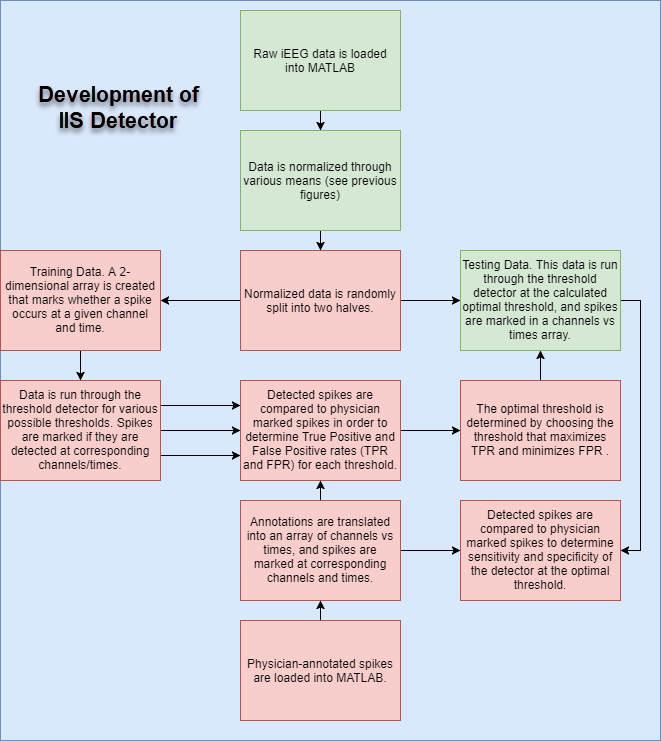
\includegraphics[height=3.5in, width=3.3in]{DetectorDevelopment.png}
    \caption{This figure depicts the full workflow for the IIS detector. All of the steps were used to develop and tune the detector, but in a clinical setting, only the green boxes would need to be applied.}
    \label{fig4}
\end{figure}


\section{RESULTS}
Fig.~\ref{fig5} contains ROC curves for the seven patients. They have been consolidated into the single red curve by computing a weighted average based on number of IISs per patient. The optimal threshold from this data, which aims to both minimize the false positive rate and maximize the true positive rate, occurs at -.46. In other words, our detector yielded the most accurate results when it marked any data that deviated by more than .46 from the normalized baseline as a spike. The automated IIS detection algorithm that we have discussed throughout this paper has, on average, a true positive rate of 98.8\% and a false positive rate of 2\%, which speaks to the accuracy of the algorithm as a reliable and independent IIS detector. 

With such a high true positive rate, we can conclude that the algorithm is very sensitive. With such a low false positive rate, we can conclude that the algorithm is also very specific in its detection of IISs. Quantifying the sensitivity and specificity of the algorithm in this way not only allows us to assess the performance of the algorithm, but also reveals how useful of a diagnostic tool this algorithm would be in identifying IISs. Additionally, one pass of the algorithm through a single hour of data requires approximately thirteen seconds to run, which is fast enough to translate its use into real-time detection. However, even if the algorithm is not currently applied in real-time, its potential as a simple numerical assessment tool is evident by its performance.

\begin{figure}
    \centering
    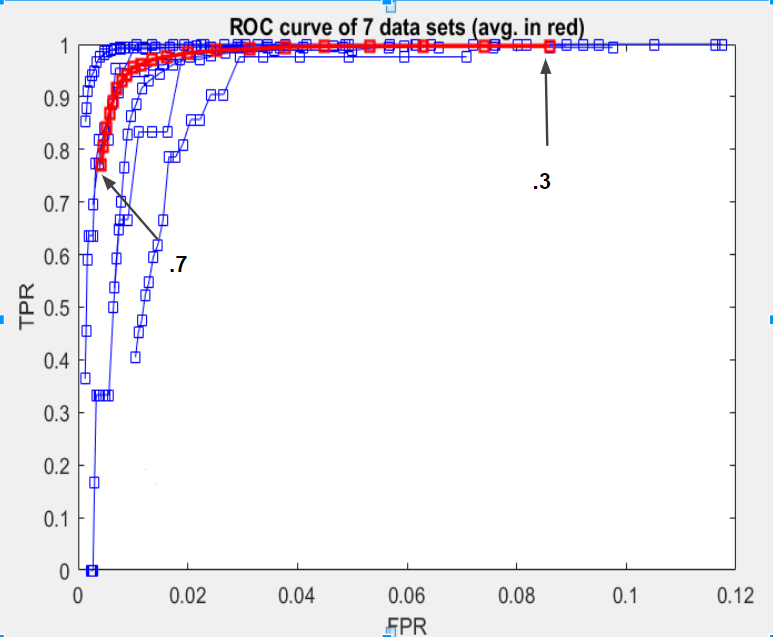
\includegraphics[scale = .42]{ROC.png}
    \caption{ROC Curves for each individual patient as well as for the consolidation of all spikes for the seven patients, shown in red. At the optimal threshold of -.46, the TPR was 98.8\% and the FPR was 2\%.}
    \label{fig5}
\end{figure}

Table~\ref{subjects} summarizes results for each patient. Our IIS detection algorithm appears to work consistently across patients with electrodes implanted in various regions of the brain.

\begin{table}
\caption{Patient Information: R=right hemisphere, L=left hemisphere F=frontal lobe, T=temporal lobe, P=Parietal lobe}
\label{table_example}
\begin{center}
\begin{tabular}{|c||c||c||c||c|}
\hline
 ID & Implantation Lobes & \# of IIS & TPR & FPR\\
\hline
m10 & R F T %RLT, RPT, RMT
& 434 & .991 & .008\\
\hline
m19 & L T P & 287 & .993 & .030\\  %LLT, LSF, LPT, LMT
\hline
m23 & R T& 347 & .994 & .008\\  %RMT, RLT, RIF, RPT
\hline
m30 & R T & 42 & .976 & .029\\ %RAT, ROT, RPT, RMT, RST
\hline
m32 & L F T & 177 & .983 & .027\\ 
%LSF, LIT, LPT, LLF, LMT
\hline
m36 & L T & 22 & 1.00 & .011\\ %LSF, LIT, LPT, LLF, LMT 
\hline
m40 & L T & 6 & 1.00 & .019\\ %LMT, LLT, LC 
\hline
\end{tabular}
\end{center}
\label{subjects}
\end{table}

%Table~\ref{subjects} summarizes results per patient.
%\begin{table*}
%\caption{Patient Information}
%\label{table_example}
%\begin{center}
%\begin{tabular}{|c||c||c||c||c|}
%\hline
% ID & Implantation  & \# of IIS & TPR & FPR\\
%\hline
%m10 & R FT right superior frontal, right lateral temporal, and right orbito-frontal %RLT, RPT, RMT
%lobes; & 434 & .991 & .008\\
%\hline
%m19 & left anterior temporal and left posterior temporal lobes& 287 & .993 & .030\\  %LLT, LSF, LPT, LMT
%\hline
%m23 & right posterior temporal and right lateral temporal lobes& 347 & .994 & .008\\  %RMT, RLT, RIF, RPT
%\hline
%m26(unused) & right superior frontal, right orbito-frontal& 24 & .958 & .168\\ %RF, RSF, RPF, RFC 
%\hline
%m30 & right mesial temporal lobe& 42 & .976 & .029\\ %RAT, ROT, RPT, RMT, RST
%\hline
%m32 & left subfrontal, left posterior temporal, and left inferior temporal lobes& 177 & .983 & .027\\ 
%%LSF, LIT, LPT, LLF, LMT
%\hline
%m36 & left posterior temporal, and left inferior temporal lobes& 22 & 1.00 & .011\\ %LSF, LIT, LPT, LLF, LMT 
%\hline
%m40 & left mesial temporal, left lateral temporal & 6 & 1.00 & .019\\ %LMT, LLT, LC 
%\hline
%\end{tabular}
%\end{center}
%\label{subjects}
%\end{table*}


\section{Discussion}
Throughout the course of this study, we have reviewed the development and implementation of an automated IIS detection algorithm derived from intracranial EEG data from seven patients that presented with epilepsy. The results of this work detailed the accuracy of the algorithm and its ability to reliably detect IISs as compared to those detected manually by an expert physician. Furthermore, it reveals that a simple threshold detector, when used in conjunction with preprocessing of iEEG data, can yield comparable results to more complex detectors. Future directions of work should involve extending this algorithm's use in real-time such that physicians can observe IISs as they occur and testing the algorithm's robustness using a wider sample of patient data. As a real-time detection method, this algorithm would enable physicians to understand the pathophysiological consequences of IISs and their relationship to epileptogenesis, providing information about when and where seizures begin in a given patient; and may eventually be useful in suppressing seizures via electrical stimulation via feedback control principles~\cite{ehrens}.


\begin{thebibliography}{99}

\bibitem{c1}  Alarcon, G., Garcia Seoane, J.J., Binnie, C.D., Martin Miguel, M.C., Juler, J., Polkey, C.E., Elwes, R.D.C., and Ortiz Blasco, J.M. (1997). Origin and propagation of interictal discharges in the acute electrocorticogram. Brain 120, 2259 - 2282.
\bibitem{c2}	Azhar F, Vendrame M, Loddenkemper T, Reinsberger C, Parkerson KA, Anderson WS. (2011). Intracranial interictal spike detection using pattern adapted wavelet methods. Abstracts of the American Epilepsy Society
\bibitem{c3}  Brown III, M.W., Porter, B.E., Dlugos, D.J., Keating, J., Gardner, A.B., Storm Jr., P.B., and Marsh, E.D. (2007). Comparison of novel computer detectors and human performance for spike detection in intracranial EEG. Clin. Neurophysiol. 118, 1744-1752.
\bibitem{c4}  El-Gohary M, McNames J, Elsas S-M. (2008). User-Guided Interictal Spike Detection. Annual International Conference of the IEEE Engineering in Medicine and Biology Society.
\bibitem{c5}  Gotman, J., and Gloor, P. (1976). Automatic recognition and quantification of interictal epileptic activity in the human scalp EEG. Electroencephalogr. Clin. Neurophysiol. 41, 513-529.
\bibitem{c6} Gaspard N, Alkawadri R, Farooque P, Goncharova II, Zaveri HP. (2014). Automatic detection of prominent interictal spikes in intracranial EEG: Clin. Neurophysiol.
\bibitem{c7} Louis, Erik K. St. (1970). Electroencephalography (EEG): An Introductory Text and Atlas of Normal and Abnormal Findings in Adults, Children, and Infants
\bibitem{c8} Pang C.C., Upton A.R., Shine G., Kamath M.V. (2003). "A Comparison of Algorithms for Detection of spikes in the Electroencephalogram", IEEE transactions on Biomedical Engineering, vol. 50, no. 4.
\bibitem{c9} Staley, Kevin J, et al. (2011). “Interictal Spikes: Harbingers or Causes of Epilepsy?” Neuroscience Letters
\bibitem{c10} Tarassenko, L., Khan Y.U., Holt M.R.G. (1998). “Identification of
inter-ictal spikes in the EEG using neural network analysis,” Inst. Elect.
Eng.—Proc. Sci. Meas. Technol., vol. 145, no. 6, pp. 270–278,
\bibitem{c11} Valenti, P., Cazamajou, E., Scarpettini, M., Aizemberg, A., Silva, W., and Kochen, S. (2006). Automatic detection of interictal spikes using data mining models. J. Neurosci. Methods 150, 105-110.
\bibitem{c12}  Wilson, S.B., and Emerson, R. (2002). Spike detection: a review and comparison of algorithms. Clin. Neurophysiol. 113, 1873-1881.
\bibitem{ehrens}
D Ehrens, D Sritharan, SV Sarma (2015) Closed-loop control of a fragile network: application to seizure-like dynamics of an epilepsy model. Frontiers in neuroscience 9, 58.

\end{thebibliography}
\addtolength{\textheight}{-3cm}   % This command serves to balance the column lengths
                                  % on the last page of the document manually. It shortens
                                  % the textheight of the last page by a suitable amount.
                                  % This command does not take effect until the next page
                                  % so it should come on the page before the last. Make
                                  % sure that you do not shorten the textheight too much.

\end{document}